
%(BEGIN_QUESTION)
% Copyright 2015, Tony R. Kuphaldt, released under the Creative Commons Attribution License (v 1.0)
% This means you may do almost anything with this work of mine, so long as you give me proper credit

Control valve FV-733 refuses to open, even with flow controller FC-733 placed in manual mode at 100\% output.  Suppose you use a voltmeter to measure DC voltage between terminal blocks 15 and 16 in the Isomerization unit shelter, and obtain a reading of 0 volts:

$$\includegraphics[width=15.5cm]{i0009rx01.eps}$$

Identify the likelihood of each specified fault for this circuit.  Consider each fault one at a time (i.e. no coincidental faults), determining whether or not each fault could independently account for {\it all} measurements and symptoms in this circuit.

% No blank lines allowed between lines of an \halign structure!
% I use comments (%) instead, so that TeX doesn't choke.

$$\vbox{\offinterlineskip
\halign{\strut
\vrule \quad\hfil # \ \hfil & 
\vrule \quad\hfil # \ \hfil & 
\vrule \quad\hfil # \ \hfil \vrule \cr
\noalign{\hrule}
%
% First row
{\bf Fault} & {\bf Possible} & {\bf Impossible} \cr
%
\noalign{\hrule}
%
% Another row
Field cable FV-733 failed open &  &  \cr
%
\noalign{\hrule}
%
% Another row
Field cable FV-733 failed shorted &  &  \cr
%
\noalign{\hrule}
%
% Another row
Cable ISOM-18 pair 4 failed open &  &  \cr
%
\noalign{\hrule}
%
% Another row
Cable ISOM-18 pair 4 failed shorted &  &  \cr
%
\noalign{\hrule}
%
% Another row
Cable ISOM-18 pair 5 failed open &  &  \cr
%
\noalign{\hrule}
%
% Another row
Cable ISOM-18 pair 5 failed shorted &  &  \cr
%
\noalign{\hrule}
%
% Another row
Cable AM9 pair 12 failed open &  &  \cr
%
\noalign{\hrule}
%
% Another row
Cable AM9 pair 12 failed shorted &  &  \cr
%
\noalign{\hrule}
%
% Another row
Cable AM14 triad 8 failed open &  &  \cr
%
\noalign{\hrule}
%
% Another row
Cable AM14 triad 8 failed shorted &  &  \cr
%
\noalign{\hrule}
%
% Another row
Failed FTA-AO control system module &  &  \cr
%
\noalign{\hrule}
%
% Another row
Direct instead of reverse controller action &  &  \cr
%
\noalign{\hrule}
%
% Another row
Diode failed open &  &  \cr
%
\noalign{\hrule}
%
% Another row
Diode failed shorted &  &  \cr
%
\noalign{\hrule}
} % End of \halign 
}$$ % End of \vbox

Suppose a fellow instrument technician suggests you connect a loop calibrator to the input terminals of FV-733 and try to ``stroke'' the control valve as a next test.  Do you think this would be a good test to do next?  Explain why or why not.

\vskip 20pt \vbox{\hrule \hbox{\strut \vrule{} {\bf Suggestions for Socratic discussion} \vrule} \hrule}

\begin{itemize}
\item{} Identify which fundamental principles of electric circuits apply to each step of your analysis of this circuit.  In other words, be prepared to explain the reason(s) ``why'' for every step of your analysis, rather than merely describing those steps.
\end{itemize}

\underbar{file i03404}
%(END_QUESTION)





%(BEGIN_ANSWER)


%(END_ANSWER)





%(BEGIN_NOTES)

FV-733 will not open, 0 volts between terminals 15 and 16:

% No blank lines allowed between lines of an \halign structure!
% I use comments (%) instead, so that TeX doesn't choke.

$$\vbox{\offinterlineskip
\halign{\strut
\vrule \quad\hfil # \ \hfil & 
\vrule \quad\hfil # \ \hfil & 
\vrule \quad\hfil # \ \hfil \vrule \cr
\noalign{\hrule}
%
% First row
{\bf Fault} & {\bf Possible} & {\bf Impossible} \cr
%
\noalign{\hrule}
%
% Another row
Field cable FV-733 failed open &  & $\surd$ \cr
%
\noalign{\hrule}
%
% Another row
Field cable FV-733 failed shorted & $\surd$ &  \cr
%
\noalign{\hrule}
%
% Another row
Cable ISOM-18 pair 4 failed open &  & $\surd$ \cr
%
\noalign{\hrule}
%
% Another row
Cable ISOM-18 pair 4 failed shorted &  & $\surd$ \cr
%
\noalign{\hrule}
%
% Another row
Cable ISOM-18 pair 5 failed open &  & $\surd$ \cr
%
\noalign{\hrule}
%
% Another row
Cable ISOM-18 pair 5 failed shorted & $\surd$ &  \cr
%
\noalign{\hrule}
%
% Another row
Cable AM9 pair 12 failed open & $\surd$ &  \cr
%
\noalign{\hrule}
%
% Another row
Cable AM9 pair 12 failed shorted & $\surd$ &  \cr
%
\noalign{\hrule}
%
% Another row
Cable AM14 triad 8 failed open &  & $\surd$ \cr
%
\noalign{\hrule}
%
% Another row
Cable AM14 triad 8 failed shorted &  & $\surd$ \cr
%
\noalign{\hrule}
%
% Another row
Failed FTA-AO control system module & $\surd$ &  \cr
%
\noalign{\hrule}
%
% Another row
Direct instead of reverse controller action &  & $\surd$ \cr
%
\noalign{\hrule}
%
% Another row
Diode failed open &  & $\surd$ \cr
%
\noalign{\hrule}
%
% Another row
Diode failed shorted &  & $\surd$ \cr
%
\noalign{\hrule}
} % End of \halign 
}$$ % End of \vbox

Attempting to stroke the valve directly using a loop calibrator (in {\it source} mode) connected to the valve's terminals (disconnecting cable FV-733 first, of course) is not a good test because we already know from the voltage readings that an electrical problem already exists preventing signal from reaching the valve.  Driving a signal to the valve positioner would check the positioner's functionality without revealing any more data about the location or nature of the electrical fault we know exists outside of the positioner.




\vskip 20pt \vbox{\hrule \hbox{\strut \vrule{} {\bf Virtual Troubleshooting} \vrule} \hrule}

This question is a good candidate for a ``Virtual Troubleshooting'' exercise.  Presenting the diagram to students, you first imagine in your own mind a particular fault in the system.  Then, you present one or more symptoms of that fault (something noticeable by an operator or other user of the system).  Students then propose various diagnostic tests to perform on this system to identify the nature and location of the fault, as though they were technicians trying to troubleshoot the problem.  Your job is to tell them what the result(s) would be for each of the proposed diagnostic tests, documenting those results where all the students can see.

During and after the exercise, it is good to ask students follow-up questions such as:

\begin{itemize}
\item{} What does the result of the last diagnostic test tell you about the fault?
\item{} Suppose the results of the last diagnostic test were different.  What then would that result tell you about the fault?
\item{} Is the last diagnostic test the best one we could do?
\item{} What would be the ideal order of tests, to diagnose the problem in as few steps as possible?
\end{itemize}


%INDEX% Documentation, loop diagram: realistic industrial example (shared by i03404 and i03891)
%INDEX% Troubleshooting review: electric circuits

%(END_NOTES)

